\documentclass[a4paper,titlepage]{scrartcl}
\pagestyle{plain}
\usepackage[utf8]{inputenc}
\usepackage[T1]{fontenc}
\usepackage[german]{babel}
\usepackage{float}
\usepackage{graphicx}
\usepackage{amsmath,amssymb,amstext}
\usepackage{enumerate}
\usepackage{units}

\numberwithin{equation}{section}

\title{Versuch P2-13: Interferenz\\Vorbereitung}
\author{Gruppe Di-22\\Jonas Müller, Genti Saliu}
\date{20. Mai 2014}

\begin{document}
	\begin{titlepage}
		\maketitle
		\thispagestyle{empty}
	\end{titlepage}
	
\newpage
\pagenumbering{roman}
\tableofcontents

\newpage
\pagenumbering{arabic}

\section{Newtonsche Ringe}
\subsection{Bestimmung vom Krümmungsradius einer symmetrischen sphärischen Bikonvexlinse}
In diesem Versuch sollte durch Beobachtung Newtonscher Ringe der Krümmungsradius $R$ einer symmetrischen sphärischen Bikonvexlinse bestimmt werden.\\ \\
Die hierzu benötigten Geräte sind \emph{Mikroskop}, Lichtquelle, hier \emph{eine einfarbige LED}, ein \emph{planer Objektträger} und \emph{die Linse}. Die Versuchsanordnung (für eine plankonvexe Linse) ist in Abbildung \ref{fig:aufgabe11} gegeben.
\begin{figure}[H]
	\centering
	\begin{tabular}{@{}r@{}}
		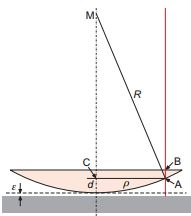
\includegraphics[width=0.4\textwidth]{bilder/aufgabe11.JPG}\\
		\footnotesize\sffamily\textbf{Quelle:} Eichler-Kronfeld-Sahm \cite{eichler}, Seite 409
	\end{tabular}
	\caption{Versuchsanordnung zur Beobachtung Netwonscher Ringe bei einer plankonvexen Linse}
	\label{fig:aufgabe11}
\end{figure}
Newtonsche Ringe entstehen, wenn man eine Linse von sehr großem Krümmungsradius auf eine planparallele Platte legt und im reflektierenden Licht beobachtet wird. In unserem Versuch dient der plane Objektträger auf dem Objekttisch des Mikroskops als planparallele Platte. Die Lichtquelle (LED) wird vorne am Mikroskop über einen Strahlteiler eingekoppelt, die Anordnung wird dabei senkrecht von oben beleuchtet.\\ \\
Die Lichtstrahlen treffen die Linse im Punkt B, dabei wird ein Teil reflektiert und ein Teil geht durch und wird erst im Punkt A weiter aufgespaltet. Hier wird wieder ein Teil der Intensität reflektiert, ein weiterer Teil durchläuft jedoch die Strecke $d + \epsilon$ und wird erst an der planparallelen Platte reflektiert. Durch diese Reflexion (am dichteren Medium) entsteht ein Phasensprung von $\pi$, den wir mit $\frac{\lambda}{2}$ bezeichnen. In Punkt A treffen die reflektierten Anteile zusammen, sie sind kohärent (gleiche Frequenz, aber mit einem Gangunterschied). Der Gangunterschied beträgt:
\begin{equation}
\label{eq:gl1}
s=2(d+\epsilon)+ \frac{\lambda}{2}=2d + \frac{\lambda}{2} \quad \text{für} \quad \epsilon=0
\end{equation}
Bei dem Zusammentreffen ensteht eine Interferenz der Lichtwellen: ist die Interferenz konstruktiv, so entstehen helle, ist sie destuktiv, dunkle Ringe. Das im Versuch zu erwartende Bild ist ähnlich wie Abbildung \ref{fig:netwon}.
\begin{figure}[H]
	\centering
	\begin{tabular}{@{}r@{}}
		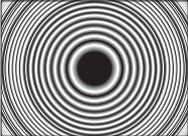
\includegraphics[width=0.3\textwidth]{bilder/newton.JPG}\\
		\footnotesize\sffamily\textbf{Quelle:} Eichler-Kronfeld-Sahm \cite{eichler}, Seite 409
	\end{tabular}
	\caption{Newtonsche Ringe in reflektiertem monochromatischen Licht}
	\label{fig:netwon}
\end{figure}
Wir wollen nun einen Zusammenhang des Beobachteten, also vom $k.$ (Nummer des dunklen Kreises vom Zentrum aus gezählt) Radius $r$ der dunkeln Ringe, vom gesuchten Krümmungsradius der Linse $R$ und von der Wellenlänge $\lambda$ des Lichtes im Ring herleiten \cite{wiki:newtonRinge}.\\ \\
Bei destruktiver Interferenz ist der Weg ein ungerades Vielfaches der halben Wellenlänge:
\begin{equation}
\label{eq:gl2}
s=(2k+1)\frac{\lambda}{2}
\end{equation}
Gleichsetzen von Gleichung \ref{eq:gl1} und \ref{eq:gl2} ergibt:
\begin{equation}
\label{eq:gl3}
2d + \frac{\lambda}{2}=(2k+1)\frac{\lambda}{2} \quad \Rightarrow \quad 2d=k\lambda
\end{equation}
Der Höhensatz von Euklid \cite{wiki:euklid} ergibt:
\begin{equation*}
r^2=2dR
\end{equation*}
Da $d \ll R$:
\begin{equation*}
r^2=2dR \quad \Rightarrow \quad d=\frac{r^2}{2R}
\end{equation*}
Einsetzen in Gleichung \ref{eq:gl3}:
\begin{equation}
\label{eq:gl5}
2 \frac{r^2}{2R}=k \lambda \quad \Rightarrow \quad \frac{r^2}{R}=k \lambda \quad \Rightarrow \quad r=\sqrt{k \lambda R}
\end{equation}
Bei der Wellenlänge muss das Brechungsindex vom Medium berücksichtigt werden, in dem Licht sich ausbreitet, also von der Luft. Es gilt:
\begin{equation}
\label{eq:gl4}
\lambda=\frac{\lambda_0}{n_L} \quad \Rightarrow \quad r_L=\sqrt{k \frac{\lambda_0}{n_L} R}
\end{equation}
Also müssen zur Bestimmung des Krümmungsradius die Radien vieler dunkler Ringe gemessen werden (vielleicht bis $k=100$) und durch Bestimmung der Steigung der Regressionsgerade der Krümmungsradius bestimmt werden.\\ \\
Die übrigen Reflexionen spielen keine Rolle für das Auftreten von Interferenzerscheinigungen, da deren Intensität sehr gering und somit vernachlässigbar ist.\\
Bei einer Durchlichtbeleuchtung hätten wir den wesentlichen Nachteil, dass das reflektierente Licht eine derart starke Intensität haben würde, dass man die dunklen Ringe nicht mehr erkennen könnte.
\subsection{Bestimmung des Brechungsindizes von Wasser}
Es soll in diesem Versuch das Brechungsindex von Wasser anhand der veränderten Radien der Netwonschen Ringen bestimmt werden. Die Versuchsanordnung bleibt gleich wie in Aufgabe 1.1, jedoch soll sich nun zwischen Linse und Objektträger (planparallele Platte) Wasser befinden.\\ \\
Es gilt:
\begin{equation*}
\lambda_{W}=\frac{\lambda_0}{n_{W}}
\end{equation*}
Einsetzen in Gleichung \ref{eq:gl4} ergibt:
\begin{equation}
\label{eq:gl6}
r_{W}=\sqrt{k \frac{\lambda_0}{n_{W}} R} \quad \Rightarrow \quad n_{W}=\frac{k \lambda_0 R}{r_{W}^2}
\end{equation}
Aus Gleichung \ref{eq:gl5} erhalten wir:
\begin{equation*}
k R = r_L \frac{n_L}{\lambda_0}
\end{equation*}
Da in den beiden Versuchen $k$ und der Krümmungsradius sich nicht verändern, können wir die obige Beziehung in Gleichung \ref{eq:gl6} einsetzen und bekommen:
\begin{equation*}
n_{W}=\frac{r_L^2}{r_W^2} \cdot n_L
\end{equation*}
\subsection{Bestimmung der Brennweite der Linse durch Autokollimation}
Es soll nun die Brennweite $f$ der Linse mittels Autokollimation bestimmt werden. Dazu wird hinter der Linse ein Planspiegel gestellt und davor ein selbstleuchtender Gegenstand gestellt. Dabei soll der Gegenstand verschoben werden, bis sein Schatten auf sich selbst scharf aber seitenverkehrt abgebildet wird.
\begin{figure}[H]
	\centering
	\begin{tabular}{@{}r@{}}
		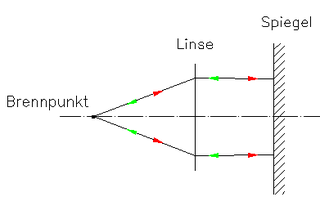
\includegraphics[width=0.5\textwidth]{bilder/autokollimation.png}\\
		\footnotesize\sffamily\textbf{Quelle:} Wikipedia \cite{wiki:autokollimation}
	\end{tabular}
	\caption{Autokollimation}
	\label{fig:aufgabe13}
\end{figure}
Der Abstand Gegenstand-Linse (in Abbildung \ref{fig:aufgabe13} befindet sich der selbstleuchtende Gegenstand im Brennpunkt) entspricht der gesuchten Brennweite $f$ der Linse.
\subsection{Bestimmung der Brechungsindex des Linsenglases aus $R$ und $f$}
Es soll in diesem Versuch das Brechungsindex des Linsenglases aus den zuvor bestimmten Krümmungsradius $R$ und Brennweite $f$ ermittelt werden. Dabei soll die Formel $R=2(n-1)f$ benutzt werden.\\ \\
Wir verifizieren nachfolgend den obigen Zusammenhang mit den Näherungen ''sehr dünne Linse'' und ''sehr achsennahe Strahlen'' (Ansatz nach \cite{wiki:naeherungduennelinse}).\\ \\
Die Linsengleichung lautet:
\begin{equation}
\label{gl:9}
\frac{1}{b}+\frac{1}{g}=\frac{1}{f}
\end{equation}
wobei $b$ Bildweite, $g$ Gegenstandsweite und $f$ die Brennweite der Linse.\\ \\
Es besteht folgender Zusammenhang zwischen Brennweite $f$, Dicke $d$ und Krümmungsradien $R_1$ bzw. $R_2$ einer bikonvexen Linse:
\begin{equation*}
\frac{1}{f}=\frac{n_2-n_1}{n_1} \left( \frac{1}{R_1}-\frac{1}{R_2} \right) + \frac{(n_2-n_1)^2 d}{n_2 n_1 R_1 R_2}
\end{equation*}
Für sehr dünne Linsen gilt $d \approx 0$, also:
\begin{equation}
\label{gl:8}
\frac{1}{f}=\frac{n_2-n_1}{n_1} \left(\frac{1}{R_1}-\frac{1}{R_2} \right)
\end{equation}
Weiterhin gilt für achsenparallele Strahen $g=\infty$ (Gegenstand liegt im Unendlichen) und $b=f$. Damit:
\begin{equation*}
\frac{1}{f}=(n_2-n_1) \left(\frac{1}{R_1}-\frac{1}{R_2} \right)
\end{equation*}
Da $R_1=R=-R_2$, folgt:
\begin{equation}
\frac{1}{f}=(n_2-n_1) \left(\frac{1}{R}+\frac{1}{R} \right)=(n_2-n_1) \frac{2}{R} \quad \Rightarrow \quad R=2(n_2-n_1)f
\end{equation}
Da das eine Material die Luft ist, beträgt $n_1 \approx 1$ und wir erhalten die zu verifizierende Relation:
\begin{equation*}
R=2(n-1)f
\end{equation*}

\section{Beugung am Gitter}
\subsection{Justieren des Gitterspektrometers}
In diesem Versuch wird ein Gitterspektrometer benutzt. Diese Besteht aus einem festen Spaltrohr (welches in der Länge variiert werden kann), einem verstellbaren Fernrohr und einem drehbaren Teilkreis. Der Teilkreis und das Fernrohr besitzen die selbe Achse um die sie gedreht werden können. Der Teilkreis ist mit Gradmarkierungen versehen so dass die Position des Fernrohrs genau bestimmt werden kann. Im Spaltrohr ist noch ein Achromat  eingebaut, welcher die chromatische Apperation möglichstklein halten soll. Am anderen Ende befindet sich der einstellbare Spalt.
 
\begin{itemize}
\item Zuerst soll die Brennweite des Fernrohrs auf "unendlich" gestellt werden, sodass der Parallaxefehler verschwindet. Für Kurzsichtige ohne Brille müssen die Einstellungen leicht geändert werden.
 
\item Nun wird der Spalt mit einer Natriumdampflampe beleuchtet. Wenn nötig wird ein Kondensor genutzt um die Lichtstrahlen parallel verlaufen zu lassen. Der Spalt wird dann so eingestellt (durch verschiebe), dass er durch das Fernrohr scharf zu erkennen ist. Jetzt wird ein Spiegel senkrecht zum Strahl in einem Gitterhalter befestigt. Zwischen Spalt und Lampe wird nun ein Objektträger so unter $45^\circ$ gegen die Achse aufgestellt, dass über diesen Strahlleiter das Licht welches vom Spiegel reflektiert wird, sichtbar ist. Zum Schluss wird dann der Spiegel gegen das Gitter getauscht.
\end{itemize}
 
\subsection{Bestimmung der Gitterkonstante}
 
Das ''Gitter'' ist eine lichtundurchlässiges Blättchen, welches von etwa 600 lichtdurchlässigen Spalten durchzogen ist. In diesem versuch nutzen wir das gelbe Licht einer Natriumdampflampe mit der mittleren Wellenlänge $\lambda = 589,3 nm$. Für die Gitterkonstante $g$ gilt $\frac{b}{g}= 0.9$ wobei b die Spaltbreite bezeichnet. Wir gehen davon aus, dass nur die Wellenlänge bekannt ist. Es gilt dann für die Minima :
 
\begin{equation}
\sin{\alpha_n}= \frac{n \cdot \lambda}{b}
\end{equation}
 
bzw. für die Maxima:
 
\begin{equation}
\sin{\alpha_n}= \frac{n \cdot \lambda}{g}
\end{equation}
 
Dabei ist n die Ordnung der Extrema. Mit den Angaben aus den Vorbereitungsunterlagen erhalten wir dann für $n=1$: $Max = 20.7^\circ$ und $Min = 23.1 ^\circ$,\\
und für $n=2$:  $Max = 45.0^{\circ}$ und $Min = 51.8 ^{\circ}$.\\
 
Größere Ordnungen sind nicht mehr zu sehen.
Es soll auch noch das Intensitätsverhältnis berechnet werden, wozu wir die Formel aus den Vorbereitungsunterlagen nutzen:
 
\begin{equation}
I = \left(\frac{\sin{\beta}}{\beta}\right)^2 \cdot \frac{\sin{N \Phi }^2}{\sin{\Phi}}
\end{equation}
 
mit 
\begin{equation}
 \beta = \frac{\pi b}{\lambda} \cdot \sin{\alpha}
\end{equation}
 
und
\begin{equation}
 \Phi = \frac{\pi g}{\lambda} \cdot \sin{\alpha}
\end{equation}
 
Dabei ist N die Anzahl der beleuchteten Spalten und $\alpha$ der Beobachtungswinkel. Damit erhalten wir für $n=1$, $I=3890$ und $n=2$, $I=3791$.
Man erhält Minima wenn $\sin{N \Phi}$ oder $ \sin{\beta}$ Null sind.
Um die Winkelauflösung zu erhalten wird der Abstand zwischen den Minima überprüft:
 
\begin{equation}
1+ N \frac{g \sin{\alpha}}{\lambda} = N \frac{g \sin{\alpha +  \Delta \alpha}}{\lambda}
\end{equation}
 
Mit den Winkelbeziehungen der Maxima erhalten wir:
 
\begin{equation}
\frac{\lambda}{\Delta \lambda} = n \cdot N
\end{equation}
 
Also braucht man um de Doppellinie für n=1 aufzulösen $N \approx 1.179$ Gitterspalten.
 
\subsection{Wellenlängenabstand der gelben Na-Linien}
 
Es soll der Abstand der gelben Na-Linien bestimmt werden. Dazu werden die Winkel beim auftreten von Maximas gemessen, mit folgender Formel lässt sich dann $\Delta \lambda$ bestimmen:
 
\begin{equation}
\Delta \lambda = \frac{g}{n}\left(\sin{\beta} - \sin{\alpha}\right)
\end{equation}
 
\subsection{Bestimmung der Gitterkonstanten eines unbekannten Gitters}
 
Es soll nun die Gitterkonstante eines Gitters bestimmt werden, welches mit dem ungefähren Wert $g= \frac{50}{mm}$ gekennzeichnet ist. Es sind viele Maxima erkennbar, da sich die Maxima mit $\sin{\alpha_n} = \frac{n \cdot \lambda}{g}$ berechnen. Da g sehr groß ist, kann man n oft erhöhen ohne, dass das Argument des Sinus größer als 1 wird. Würde man de komplette Breite von 36mm beleuchten so könnte man schon ab dem 1, Maximum eine Doppellinie auflösen. Bei 5mm Beleuchtung ab der 5. Ordnung.

\newpage
\bibliographystyle{plain}
\bibliography{quellen}

\end{document}
